% example.tex
\documentclass[dvisvgm]{standalone}

\usepackage{amsmath}
\usepackage[usenames,dvipsnames]{xcolor}
\usepackage{tikz}
\usetikzlibrary {arrows.meta,
                 calc,
                 positioning,
                 shapes.geometric}

 \tikzset{
        square/.style={regular polygon, regular polygon sides=4, minimum
        width=12mm},
        base/.style={draw, align=center, minimum height=4ex},
        proc/.style={base, rectangle, text width=8em},
        io/.style={trapezium, trapezium left angle=70, trapezium right
                   angle=110, draw, text width=8em, %minimum width=2cm, 
                   %minimum height=1cm
                   },
        test/.style={base, diamond, aspect=2,
                     text width=8em
                     },
        term/.style={proc, rounded corners},
        myarrow/.style={-Stealth, line width=0.25mm},
 }

\begin{document}
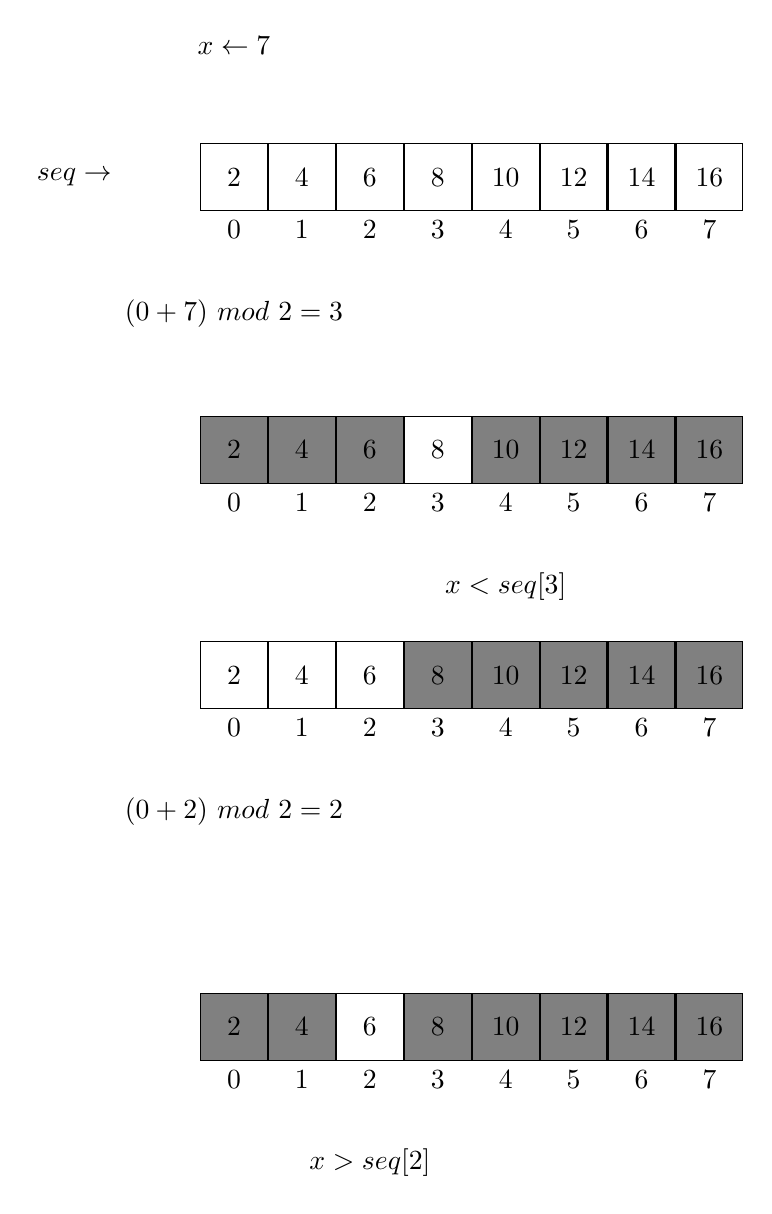
\begin{tikzpicture}
    \node[draw, square, label=below:0] (a0) {2};
    \node[draw, square, label=below:1, right=0cm of a0] (a1) {4};
    \node[draw, square, label=below:2, right=0cm of a1] (a2) {6};
    \node[draw, square, label=below:3, right=0cm of a2] (a3) {8};
    \node[draw, square, label=below:4, right=0cm of a3] (a4) {10};
    \node[draw, square, label=below:5, right=0cm of a4] (a5) {12};
    \node[draw, square, label=below:6, right=0cm of a5] (a6) {14};
    \node[draw, square, label=below:7, right=0cm of a6] (a7) {16};

    \node[left=of a0] (seq) {$seq \rightarrow$};

    \node[above= of a0] (0) {$x \leftarrow 7$};

    \node[below= of a0] (first) {$(0+7)\ mod\ 2 = 3$};


    \node[draw, square, fill=gray, label=below:0, below= of first] (b0) {2};
    \node[draw, square, fill=gray, label=below:1, right=0cm of b0] (b1) {4};
    \node[draw, square, fill=gray, label=below:2, right=0cm of b1] (b2) {6};
    \node[draw, square, label=below:3, right=0cm of b2] (b3) {8};
    \node[draw, square, fill=gray, label=below:4, right=0cm of b3] (b4) {10};
    \node[draw, square, fill=gray, label=below:5, right=0cm of b4] (b5) {12};
    \node[draw, square, fill=gray, label=below:6, right=0cm of b5] (b6) {14};
    \node[draw, square, fill=gray, label=below:7, right=0cm of b6] (b7) {16};

    \node[below= of b4] (comp1) {$x < seq[3]$};

    \node[draw, square, label=below:0, below=2cm of b0] (c0) {2};
    \node[draw, square, label=below:1, right=0cm of c0] (c1) {4};
    \node[draw, square, label=below:2, right=0cm of c1] (c2) {6};
    \node[draw, square, fill=gray, label=below:3, right=0cm of c2] (c3) {8};
    \node[draw, square, fill=gray, label=below:4, right=0cm of c3] (c4) {10};
    \node[draw, square, fill=gray, label=below:5, right=0cm of c4] (c5) {12};
    \node[draw, square, fill=gray, label=below:6, right=0cm of c5] (c6) {14};
    \node[draw, square, fill=gray, label=below:7, right=0cm of c6] (c7) {16};

    \node[below= of c0] (second) {$(0+2)\ mod\ 2 = 2$};

    \node[draw, square, fill=gray, label=below:0, below=2cm of second] (d0) {2};
    \node[draw, square, fill=gray, label=below:1, right=0cm of d0] (d1) {4};
    \node[draw, square, label=below:2, right=0cm of d1] (d2) {6};
    \node[draw, square, fill=gray, label=below:3, right=0cm of d2] (d3) {8};
    \node[draw, square, fill=gray, label=below:4, right=0cm of d3] (d4) {10};
    \node[draw, square, fill=gray, label=below:5, right=0cm of d4] (d5) {12};
    \node[draw, square, fill=gray, label=below:6, right=0cm of d5] (d6) {14};
    \node[draw, square, fill=gray, label=below:7, right=0cm of d6] (d7) {16};

    \node[below= of d2] (comp2) {$x > seq[2]$};
\end{tikzpicture}
\end{document}
